\documentclass[12pt,a4paper,twoside]{article}
\usepackage{labor}
\begin{document}

%fill for cover and header creation
\newcommand\laboratorynumber{2}
\title{Fallrohr}
\newcommand\supervisor{Ditlbacher, Harald}
\newcommand\groupnumber{42}

\newcommand\participantonelastname{Eisner}
\newcommand\participantonefirstname{Nico}
\newcommand\participantoneid{12214121}
\newcommand\participanttwolastname{Waldl}
\newcommand\participanttwofirstname{Philip}
\newcommand\participanttwoid{12214120}
\author{\participantonelastname \ \& \participanttwolastname}

\newcommand\degreeid{UB 033 678}
\newcommand\semester{23WS}
\date{18.11.2023}

%select correct course title
%\newcommand\coursetitle{Einführung in die \\ physikalischen Messmethoden}
%\newcommand\coursetitle{Laborübungen 1: \\ Mechanik und Wärme}
\newcommand\coursetitle{Laborübungen 2: \\ Elektrizität, Magnetismus, Optik}
%\newcommand\coursetitle{Fortgeschrittenen Praktikum 1: \\ Technische Physik}
%\newcommand\coursetitle{Fortgeschrittenen Praktikum 2: \\ Allgemeine Physik}

%\begin{titlepage}
   \begin{center}
       \begin{figure}[H]
            \begin{minipage}[h]{30mm}
                \centerline{
\includegraphics[height=15mm]{cover_nudes/tugraz.png}}
            \end{minipage}
            \hfill
            \begin{minipage}[h]{30mm}
                \centerline{
\includegraphics[height=15mm]{cover_nudes/nawi_graz.png}}
            \end{minipage}
            \hfill
            \begin{minipage}[h]{30mm}
                \centerline{
\includegraphics[height=15mm]{cover_nudes/uni-graz.png}}
            \end{minipage}
        \end{figure}
        
        \large{\emph{Institut für Experimentalphysik der Technischen Universität Graz \\
        \& Institut für Physik der Universität Graz}} \\
        \vspace{5mm}
        
        {\Huge \textbf{\coursetitle}}
        \vspace{5mm}
        
        {\huge \laboratorynumber: \thetitle}
    \end{center}
    
    \vfill
    
    \begin{table}[H]
        \LARGE
        \centering
        \begin{tabular}{r l}
            Betreuer:       & \supervisor \\
            Gruppennummer:  & \groupnumber \\
            \\
            Name:           & \participantonelastname, \participantonefirstname \\
            Matrikelnummer: & \participantoneid \\
            Name:           & \participanttwolastname, \participanttwofirstname \\
            Matrikelnummer: & \participanttwoid \\
            \\
            Kennzahl:       & \degreeid \\
            Datum:          & \semester \ | \thedate
        \end{tabular}
    \end{table}
    \vspace{4cm}
\end{titlepage}
\clearpage
\setcounter{page}{1}

%\maketitle %short title alternative

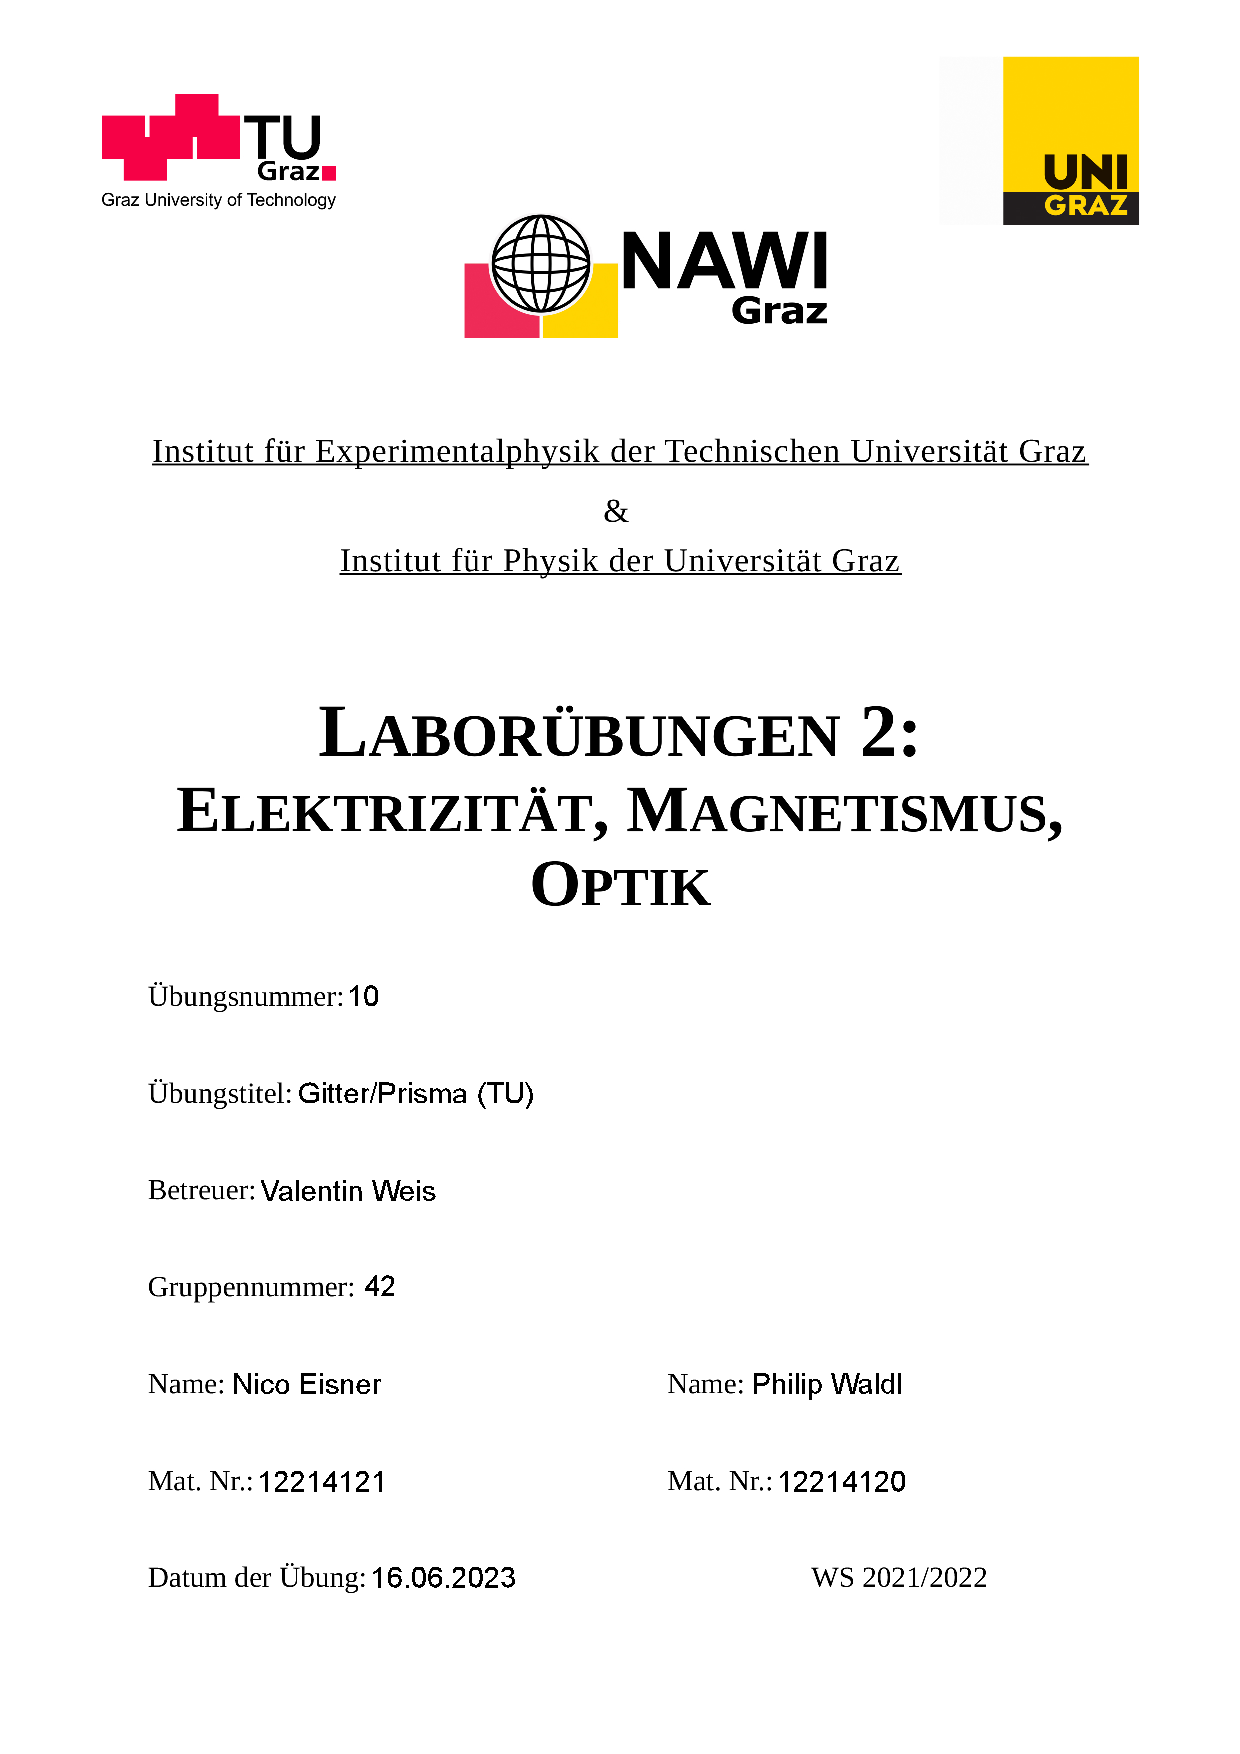
\includepdf[pages={1}]{../Deckblätter/Deckblatt_Gitter.pdf}

\tableofcontents
\newpage

\section{Aufgabenstellung} %jo beschreibn wos gmocht host ------------------------------

Der Versuche Operationsverstärker behandelt das gleichnamige Elektronikbauteil, welches in der Elektronik in erster Linie zur Verstärkung von elektrischen Signalen eingesetzt wird.
Über mehrere, verschiedene Schaltungen hinweg sollen einige Anwendungsbereiche des OPVs gezeigt und experimentell bestätigt werden.

Die genaue Aufgabenstellung sieht dabei wie folgt aus:

\begin{itemize}
    \item Aufbau der Schaltung für den Operationsverstärker (OPV)
    \item Invertierter OPV
    \begin{itemize}
        \item Verstärkung V 
        \item Phasendifferenz $\phi$ zwischen Ein- und Ausgangssingal für verschiedene Rückkopplungswiderstände $\tau$
    \end{itemize}
    \item Nichtinvertierter OPV
    \begin{itemize}
        \item Funktionsweiße des nichtinvertierten OPV für verschiedene Widerstandskombinationen
    \end{itemize}
    \item OPV als Differenzierer
    \begin{itemize}
        \item Funktionsweiße des OPV als Differenzierer für verschiedene Widerstandskombinationen und Eingangssignalarten
    \end{itemize}
    \item OPV als Integrierer
    \begin{itemize}
        \item Funktionsweiße des OPV als Integrierer für verschiedene Widerstandskombinationen und Eingangssignalarten
    \end{itemize}
\end{itemize}

\noindent
Alle Informationen und Methodiken wurden uns von der Technischen Universität bereitgestellt \cite{teachcenter2}. 


\section{Voraussetzungen \& Grundlagen} %Grundlagen erklären, Formeln mit erklärung

Wie bereits im Kapitel Aufgabenstellung eingeleitet ist der Operationsverstärker ein elektrisches Schaltelement, genauer ein gleichspannungsgekoppelter Differenzenverstärker, welcher einen invertierten- und einen nichtinvertierten Eingang besitzt. Er soll dabei die Differenz zwischen den beiden Eingangssignalen verstärken und einem idealen Verstärker (möglichst hohe Verstärkung, Eingangswiderstände und möglichst geringe Ausgangswiderstände) nahe kommen. Der grobe Aufbau eines OPVs lässt sich in folgender Abbildung \ref{fig:OpvAufbau} erkennen.

\begin{figure}[H]
    \centering
    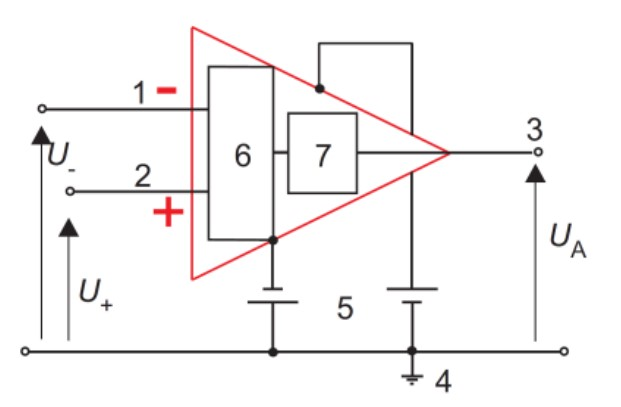
\includegraphics[width=0.6\linewidth]{nudes/OpvGrundlegenderAufbau.jpg}
    \caption{OPV grundlegender Aufbau \cite{teachcenter2}}
    \label{fig:OpvAufbau}
\end{figure}

\noindent
In Abbildung \ref{fig:OpvAufbau} lassen sich die beiden Eingänge 1 (invertiert) und 2 (nicht invertiert) und der Ausgang 3 erkennen. Weiters befindet sich im OPV (meist dargestellt als Dreieck) ein Differenzenverstärker 6 und ein Impedanzwandler 7. Für den Betrieb ist außerdem eine Spannungsversorgung 5 und ein gemeinsamer Groundpunkt 4 von nöten. \newline

\noindent
Mit dem beschriebenen Operationsverstärker lassen sich nun einige Grundschaltungen darstellen:

\subsection{Invertierender Verstärker}

Beim invertierenden Verstärker wird das Signal über den invertierten Eingang mit einem Eingagnswiderstand $R_{1}$ eingespeist und der nichtinvertierte Eingang ist auf Ground gelegt. Der Widerstand $R_{2}$ ist dabei der Rückkopplungswiderstand, welcher bestimmt, wie viel vom Ausgangssignal zurück zum Eingang fließt und das Signal verstärkt.
Das Resultat des invertierten Verstärkers ist ein verstärktes und umgekehrtes Ausgangssignal, welches vom Verhältnis der beiden Widerstände abhänge und sich somit folgend beschreiben lässt:

\begin{equation}
    \label{eq:InvertierenderVerstärkerAusgang}
    \centerline{$U_{A}=-\frac{R_{2}}{R_{1}}U_{1}$}
\end{equation}

\noindent
Die Verstärkung lässt sich dabei so ausdrücken:

\begin{equation}
    \label{eq:InvertierenderVerstärkerVerstärkung}
    \centerline{$V=-\frac{R_{2}}{R_{1}}$}
\end{equation}

\noindent
Das Schaltbild des invertierten Verstärkers lässt sich in folgender Abbildung \ref{fig:InvertierenderVerstärker} erkennen.

\begin{figure}[H]
    \centering
    \includegraphics[width=0.3\linewidth]{nudes/Invertierender Verstärker.jpg}
    \caption{Invertierender Verstärker \cite{teachcenter2}}
    \label{fig:InvertierenderVerstärker}
\end{figure}


\subsection{Nichtinvertierender Verstärker}

Der nichtinvertierende Verstärker sieht im Aufbau dem invertierenden Verstärker sehr ähnlich. Der größte Unterschied ist, dass das Eingangssignal über den nichtinvertierten Eingang mit Eingagnswiderstand kommt und der invertierte Eingang auf Masse gelegt ist.
Beim nichtinvertierenden Verstärker verlässt das Signal die Schaltung nur verstärkt, was in folgender Gleichung für die Verstärkung resultiert:

\begin{equation}
    \label{eq:NichtinvertierenderVerstärkerVerstärkung}
    \centerline{$V=1 + \frac{R_{2}}{R_{1}}$}
\end{equation}

\noindent
Der Aufbau sieht dabei wie folgt aus:

\begin{figure}[H]
    \centering
    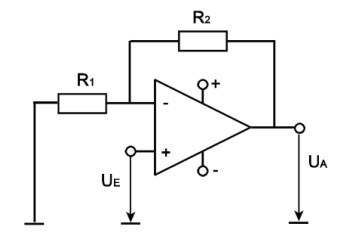
\includegraphics[width=0.3\linewidth]{nudes/Nichtinvertierender Verstärker.jpg}
    \caption{Nichtinvertierender Verstärker \cite{teachcenter2}}
    \label{fig:NichtInvertierenderVerstärker}
\end{figure}


\subsection{Addierer, Subtrahierer}

Werden zwei Eingangsspannungen mit Eingangswiderständen an den invertierten Eingang- und eine Eingangsspannung mit Spannungsteiler an den nichtinvertierten Eingang geschaltet, so erhält man einen funktionstüchtigen Addierer bzw. Subtrahierer.
Die Funktion der Schaltung ist dabei von den gewählten Widerständen abhängig und sieht im Aufbau wie folgt aus:

\begin{figure}[H]
    \centering
    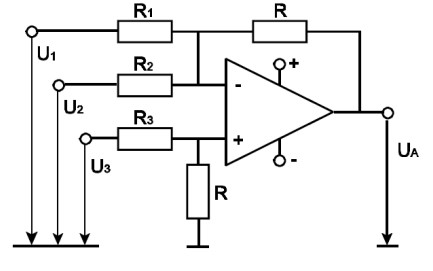
\includegraphics[width=0.3\linewidth]{nudes/AddiererSubtrahierer.jpg}
    \caption{Addierer/Subtrahierer \cite{teachcenter2}}
    \label{fig:AddiererSubtrahierer}
\end{figure}


\subsection{Differenzierer}

Des weiteren ist es möglich, unter einbezug eines Operationsverstärkers zu differenzieren. Dabei wird der invertierenden Verstärkerschaltung ein Kondensator vor dem Eingangswiderstand $R_{1}$ hinzugefügt. Anhand der Lade- bzw. Entladezeiten lässt sich so durch die zeitliche Ableitung von $Q = C*U_{E}$ die Ausgangsspannung als differenzierte Eingangsspannung definieren:

\begin{equation}
    \label{eq:DifferenziererAusgang}
    \centerline{$U_{A}=-RC \frac{\partial U_{E}}{\partial t}$}
\end{equation}

\noindent
Die hierzu nötige Schaltung ist in Abbildung \ref{fig:Integrierer} ersichtlich.

\begin{figure}[H]
    \centering
    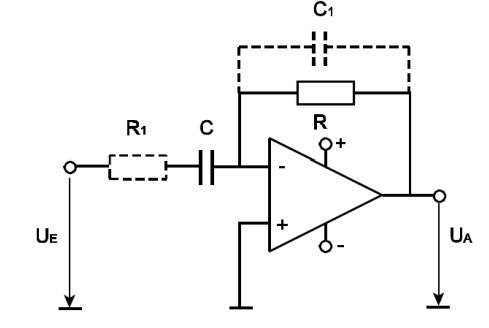
\includegraphics[width=0.3\linewidth]{nudes/Differenzierer.jpg}
    \caption{Differenzierer \cite{teachcenter2}}
    \label{fig:Differenzierer}
\end{figure}


\subsection{Integrierer}

Ähnlichem Prinzip folgt auch der Integrierer, welcher sich zum Differenzierer lediglich durch die Anordnung des Kondensators unterscheidet. Dieser wird nun nicht vor den Eingangswiderstand, sondern paralell zum Rückkopplungswiderstand geschaltet.
Dadurch erzielt man an der Ausgangsspannung die Stammfunktion der Eingangsspannung.

\begin{equation}
    \label{eq:IntegriererAusgang}
    \centerline{$U_{A}=-\frac{1}{RC} \int_{}^{} U_{E} \,dt + c $}
\end{equation}

\noindent
Aufgebaut sieht der Integrierer wie folgt aus:

\begin{figure}[H]
    \centering
    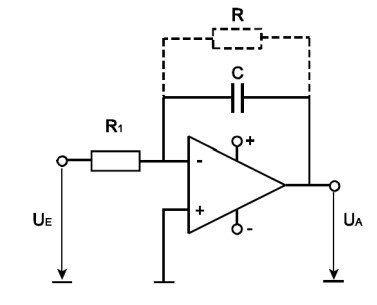
\includegraphics[width=0.3\linewidth]{nudes/Integrierer.jpg}
    \caption{Integrierer \cite{teachcenter2}}
    \label{fig:Integrierer}
\end{figure}


\section{Versuchsanordnung} %mit skizze kurz beschreiben ------------------------------

Zu Beginn des Versuches wurden zwei grundlegende Schaltungen realisiert, welche abgesehen vom Operationsverstärker noch ein bzw. zwei Potentiometer mit 100 $\Omega$, zwei Widerstände mit 47 $k \Omega$, den Funktionsgenerator und das Netzgerät mit einer Spannnung von $\pm$15 V. Der Aufbau der Schaltung ist in folgenden Abbildungen \ref{fig:GrundschaltungAufbau} ersichtlich.

\begin{figure}[H]
    \centering
    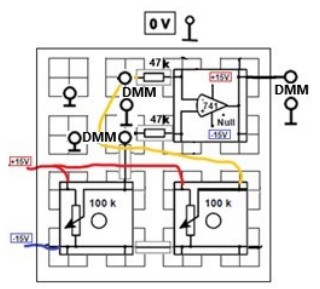
\includegraphics[width=0.4\linewidth]{nudes/GrundschaltungAufbau1.jpg}
    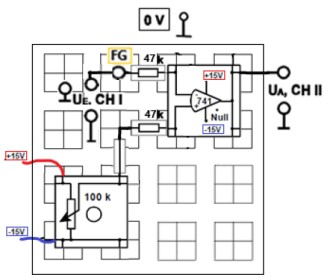
\includegraphics[width=0.4\linewidth]{nudes/GrundschaltungAufbau2.jpg}
    \caption{Grundschaltungen Aufbau \cite{teachcenter2}}
    \label{fig:GrundschaltungenAufbau}
\end{figure}

\begin{figure}[H]
    \centering
    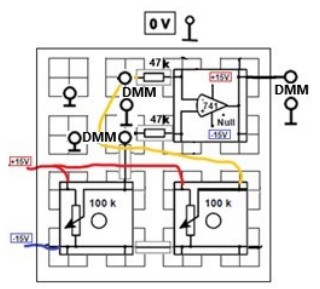
\includegraphics[width=0.4\linewidth]{nudes/GrundschaltungAufbau1.jpg}
    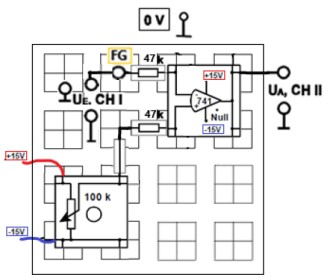
\includegraphics[width=0.4\linewidth]{nudes/GrundschaltungAufbau2.jpg}
    \caption{Grundschaltungen realer Aufbau}
    \label{fig:GrundschaltungenAufbauIRL}
\end{figure}

\noindent
Folgend dazu wurde dann der invertierende Verstärker realisiert. Der Schaltungsaufbau hierzu ist in folgenden Abbildungen zu erkennen.

\begin{figure}[H]
    \centering
    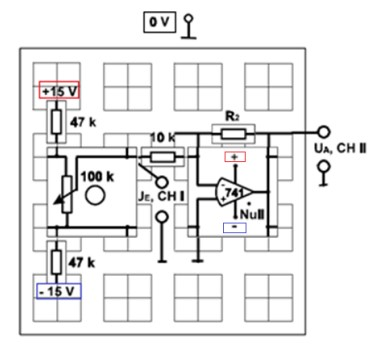
\includegraphics[width=0.4\linewidth]{nudes/InvertierenderVerstärkerSchaltungAufbau.jpg}
    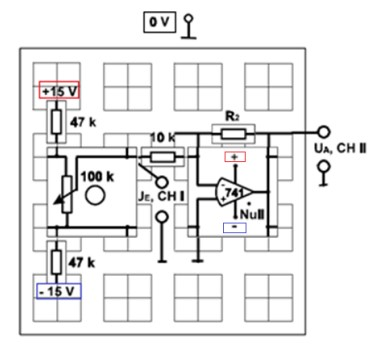
\includegraphics[width=0.4\linewidth]{nudes/InvertierenderVerstärkerSchaltungAufbau.jpg}
    \caption{Invertierender Verstärker Schaltung und realer Aufbau \cite{teachcenter2}}
    \label{fig:SchaltungInvertierenderVerstärker}
\end{figure}

\noindent
Natürlich wurde dann auch der nichtinvertierende Verstärker in Realität umgesetzt:

\begin{figure}[H]
    \centering
    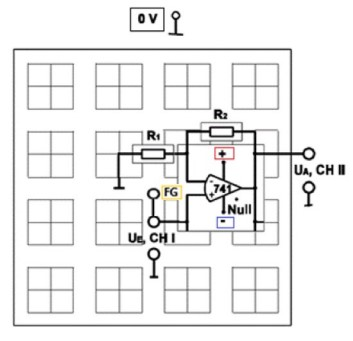
\includegraphics[width=0.4\linewidth]{nudes/NichtInvertierenderVerstärkerSchaltungAufbau.jpg}
    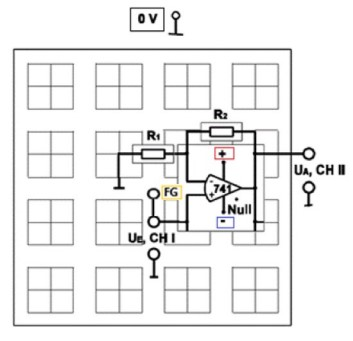
\includegraphics[width=0.4\linewidth]{nudes/NichtInvertierenderVerstärkerSchaltungAufbau.jpg}
    \caption{Nichtinvertierender Verstärker Schaltung und realer Aufbau \cite{teachcenter2}}
    \label{fig:SchaltungNichtInvertierenderVerstärker}
\end{figure}

\noindent
Am Ende des Versuches wurde es dann etwas komplexer, da nun Differenzierer und Integrierer in die Tat umgesetzt wurden. Die hierfür benötigten Schaltpläne sind in folgenden Abbildungen ersichtlich: 

\begin{figure}[H]
    \centering
    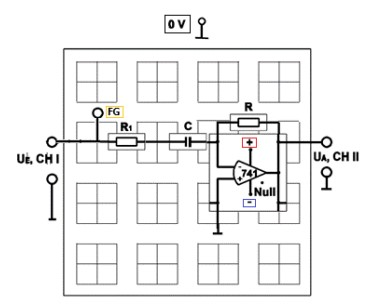
\includegraphics[width=0.4\linewidth]{nudes/DifferenziererSchaltungAufbau.jpg}
    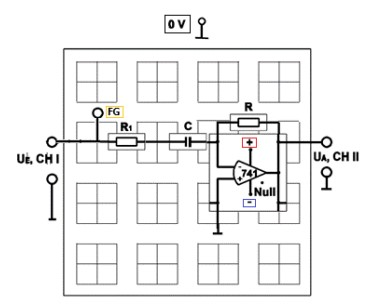
\includegraphics[width=0.4\linewidth]{nudes/DifferenziererSchaltungAufbau.jpg}
    \caption{Differenzierer Schaltung und realer Aufbau \cite{teachcenter2}}
    \label{fig:SchaltungDifferenzierer}
\end{figure}

\begin{figure}[H]
    \centering
    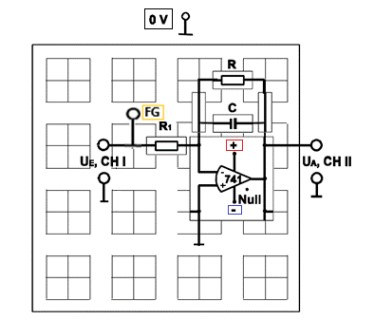
\includegraphics[width=0.4\linewidth]{nudes/IntegriererSchaltungAufbau.jpg}
    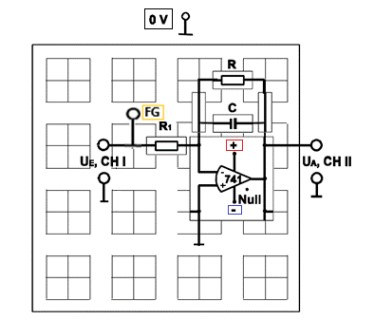
\includegraphics[width=0.4\linewidth]{nudes/IntegriererSchaltungAufbau.jpg}
    \caption{Integrierer Schaltung und realer Aufbau \cite{teachcenter2}}
    \label{fig:SchaltungIntegrierer}
\end{figure}



\section{Geräteliste} %jo holt a listn ------------------------------

    \begin{table}[H]
        \centering
        \caption{Im Versuch verwendete Geräte und Utensilien.}
        \label{tab:geraete}
        \resizebox{\columnwidth}{!}{\begin{tabular}{|l|l|l|}
            \hline
            Gerät   & Gerätenummer  & Unsicherheit \\
            \hline
            Oszilloskop                                                                          & {n.a} & {n.a} \\
            Steckboard                                                                           & {n.a} & {n.a} \\
            Widerstände (0$\Omega$, 0.1 k$\Omega$, 0.47 k$\Omega$, 1 k$\Omega$, 1.5 k$\Omega$, 
            2.2 k$\Omega$, 4.7 k$\Omega$, 10 k$\Omega$, 15 k$\Omega$, 1 M$\Omega$)               & {n.a} & $\pm$1\% \\
            Funktionsgenerator                                                                   & {n.a} & {n.a} \\
            Netzgerät                                                                            & {n.a} & {n.a} \\
            Operationsverstärker                                                                 & {n.a} & {n.a} \\
            2x Potentiometer (100 k$\Omega$)                                                     & {n.a} & $\pm$10\% \\
            3x Digitalmultimeter                                                                 & {n.a} & $\pm$1.2\% + 2 sigit\\
            Kondensatoren (10 nF, 2.2 nF, 1 $\mu F$)                                             & {n.a} & $\pm$10\% \\
            Verbindungskabel                                                                     & {n.a} & {n.a} \\
            \hline
        \end{tabular}}
    \end{table}


\section{Versuchsdurchführung \& Messergebnisse} %nachvollziehbar und klar dargestellt ------------------------------

\begin{table}[H]
    \centering
    \caption{Grundschaltung Messungen}
    \label{tab:GrundschaltungMessungen}
    \begin{tabular}{| l | l | l | l |}
        \hline
        Nr. & $U_{Ein1}$ / V & $U_{Ein2}$ / V & $U_{Aus1}$ / V \\
        \hline
        1 & -0.0461 $\pm$  & -0.789 $\pm$  & -13.15 $\pm$  \\
        2 & -0.0833 $\pm$  & -0.790 $\pm$  & -13.15 $\pm$  \\
        3 & -0.0612 $\pm$  & -0.789 $\pm$  & -13.15 $\pm$  \\
        4 & -0.1069 $\pm$  & -0.789 $\pm$  & -13.15 $\pm$  \\
        5 & -0.0890 $\pm$  & -0.790 $\pm$  & -13.15 $\pm$  \\
        \hline
    \end{tabular}
\end{table}

\begin{table}[H]
    \centering
    \caption{Invertierender OPV 10 k$\Omega$ Verstärkungen gemessen}
    \label{tab:IoVerstärkungenGemessen10}
    \begin{tabular}{| l | l | l | l |}
        \hline
        Nr. & Zieleingangsspannungen / V & $U_{Ein}$ / V & $U_{Aus}$ / V \\
        \hline
        1 &  1.5 &  1.511 $\pm$  & -1.530 $\pm$  \\
        2 &  1.0 &  1.022 $\pm$  & -1.035 $\pm$  \\
        3 &  0.5 &  0.499 $\pm$  & -0.505 $\pm$  \\
        4 &  0.0 &  0.024 $\pm$  & -0.234 $\pm$  \\
        5 & -0.5 & -0.521 $\pm$  &  0.521 $\pm$  \\
        6 & -1.0 & -1.039 $\pm$  &  1.039 $\pm$  \\
        7 & -1.5 & -1.532 $\pm$  &  1.532 $\pm$  \\
        \hline
    \end{tabular}
\end{table}

\begin{table}[H]
    \centering
    \caption{Invertierender OPV 33 k$\Omega$ Verstärkungen gemessen}
    \label{tab:IoVerstärkungenGemessen33}
    \begin{tabular}{| l | l | l | l |}
        \hline
        Nr. & Zieleingangsspannungen / V & $U_{Ein}$ / V & $U_{Aus}$ / V \\
        \hline
        1 &  1.5 &  1.486 $\pm$  & -4.950 $\pm$  \\
        2 &  1.0 &  1.011 $\pm$  & -3.358 $\pm$  \\
        3 &  0.5 &  0.511 $\pm$  & -1.706 $\pm$  \\
        4 &  0.0 &  0.010 $\pm$  & -0.031 $\pm$  \\
        5 & -0.5 & -0.511 $\pm$  &  1.699 $\pm$  \\
        6 & -1.0 & -1.013 $\pm$  &  3.368 $\pm$  \\
        7 & -1.5 & -1.496 $\pm$  &  4.980 $\pm$  \\
        \hline
    \end{tabular}
\end{table}

\begin{table}[H]
    \centering
    \caption{Invertierender OPV 100 k$\Omega$ Verstärkungen gemessen}
    \label{tab:IoVerstärkungenGemessen100}
    \begin{tabular}{| l | l | l | l |}
        \hline
        Nr. & Zieleingangsspannungen / V & $U_{Ein}$ / V & $U_{Aus}$ / V \\
        \hline
        1 &  1.5 &  1.464 $\pm$  & -13.140 $\pm$  \\
        2 &  1.0 &  1.054 $\pm$  & -10.700 $\pm$  \\
        3 &  0.5 &  0.519 $\pm$  &  -5.260 $\pm$  \\
        4 &  0.0 & -0.009 $\pm$  &  -0.094 $\pm$  \\
        5 & -0.5 & -0.493 $\pm$  &   5.010 $\pm$  \\
        6 & -1.0 & -1.036 $\pm$  &  10.530 $\pm$  \\
        7 & -1.5 & -1.656 $\pm$  &  14.330 $\pm$  \\
        \hline
    \end{tabular}
\end{table}

\begin{table}[H]
    \centering
    \caption{NichtInvertierender OPV Verstärkungen}
    \label{tab:NioVerstärkungenGemessen}
    \begin{tabular}{| l | l | l | l | l |}
        \hline
        Nr. & $R_{2}$ / $k \Omega$ & V ($\frac{Kästchen}{Kästchen}$) / & V / dB & U pro Kästchen / V \\
        \hline
        1 &  0.00 $\pm$  & $\frac{1.0}{1.0}$ =  1.000 $\pm$  &  $\pm$  & 0.5 $\pm$  \\
        2 &  0.47 $\pm$  & $\frac{2.2}{1.5}$ =  1.467 $\pm$  &  $\pm$  & 0.5 $\pm$  \\
        3 &  1.50 $\pm$  & $\frac{3.7}{1.5}$ =  2.467 $\pm$  &  $\pm$  & 0.5 $\pm$  \\
        4 &  2.20 $\pm$  & $\frac{4.8}{1.5}$ =  3.200 $\pm$  &  $\pm$  & 0.5 $\pm$  \\
        5 &  4-70 $\pm$  & $\frac{4.4}{0.7}$ =  6.290 $\pm$  &  $\pm$  & 1.0 $\pm$  \\
        6 & 10.00 $\pm$  & $\frac{4.1}{0.4}$ = 10.250 $\pm$  &  $\pm$  & 2.0 $\pm$  \\
        \hline
    \end{tabular}
\end{table}



\section{Auswertung und Unsicherheitsanalyse} %Nicht nur zahlen angeben ------------------------------

In der Auswertung werden zur erhöhten Genauigkeit durchgehend ungerundete Werte bis zu den Endergebnissen verwendet und nur zur Darstellung gerundet. \\
Zur Berechnung der Unsicherheiten wird, wenn nicht anders angegeben, die Größtunsicherheitsmethode verwendet.


\section{Diskussion} %diskussion der Unsicherheiten und Ergebnisse und evtl. verlgeich mit Literatur ------------------------------


\section{Zusammenfassung} %klare, übersichtliche vollständige beantwortung der Aufgabenstellung ------------------------------


\printbibliography[heading=bibintoc]
\end{document}
